 \documentclass{article}
\usepackage[utf8]{inputenc}
\usepackage{float}
\usepackage{amsmath}
\usepackage[labelsep=period]{caption} % Figur. istället för Figur:
\usepackage{relsize}
\usepackage{multirow}
\usepackage[export]{adjustbox}
\usepackage{subcaption}
\usepackage{wrapfig}
\usepackage{hyperref}
\usepackage{array}
\usepackage{amsmath}
\usepackage{geometry}
\usepackage{parskip}
\newcommand\tab[1][1cm]{\hspace*{#1}}

\title{Reinforcement Learning EL2805\\
       Laboration 1}

\author{Ilian Corenliussen, 950418-2438, ilianc@kth.se\\ 
        Daniel Hirsch, 960202-5737, dhirsch@kth.se}
\date{November 2020}

\begin{document}

\maketitle

\section*{Problem 1: \\
        The Maze and the Random Minotaur}
\subsection*{A)}
The problem can me modelled as an MDP such that, the number of states is depending on the grid space and the player and Minotaur position, e.g. $S = \{((P_x, H_y),(P_x, M_y) )\} $ where $P_x$ and $P_y$ is the player and $M_x$ and $M_y$ the Minotaur position x and y position within the grid. The state space can be divided into $S = {S_a, S_u}$ where $S_a$ is the allowed states and $S_u$ is the unreachable states, such as wall or out-of-boundary.


\textbf{State space:}\\
$S = \{((P_x, H_y),(P_x, M_y) )\} $, 3136 number of states. 

\textbf{Actions}: \\
The actions can be as described in the lab instructions as left, right, up, down or stay at the current position, $A = \{ A_{left}, A_{right}, A_{up}, A_{down}, A_{stay} \}$. 

\textbf{Rewards:} \\
Eaten: $r(P_x = M_x , P_y = M_y |s,a) = -100 $\\ 
Goal: $r(P_x = B_x , P_y = B_y |s,a) = 0 $, where $B_x$, $B_y$ is the goal position\\
Wall: $r(s'\in S_u |s,a) = -\infty $\\
Walking: $r(s'\in S_a |s,a) = -1 $

\textbf{Transition Probabilities}:\\
$P_t(s' \in S_a |s,a) = 1/n$, where n is the number of possible moves for the Minotaur and \\$P_t(s \in S_u |s,a) = 0$. 

\subsection*{B)}
The optimal policy of the player and the minotaur are displayed in Figure \ref{fig:Policy}, where Player: t and Minotaur: t was their respective position for the timestep t. 


\begin{figure}[H]
    \centering
    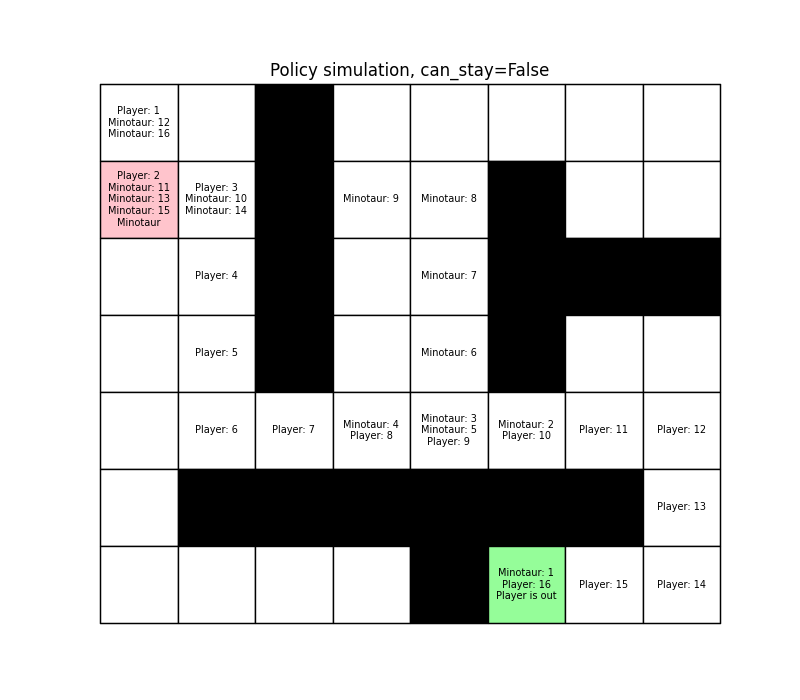
\includegraphics[width=0.8\textwidth]{Lab_1/images/problem_1/MazeRun_Nov-16-2020_11-55-45.png}
    \caption{\small Illustration of the policy for one run, where Player: 1 and Minotaur: 1 is the position for time t=1, etc. }
    \label{fig:Policy}
\end{figure}

\begin{figure}[H]
    \centering
    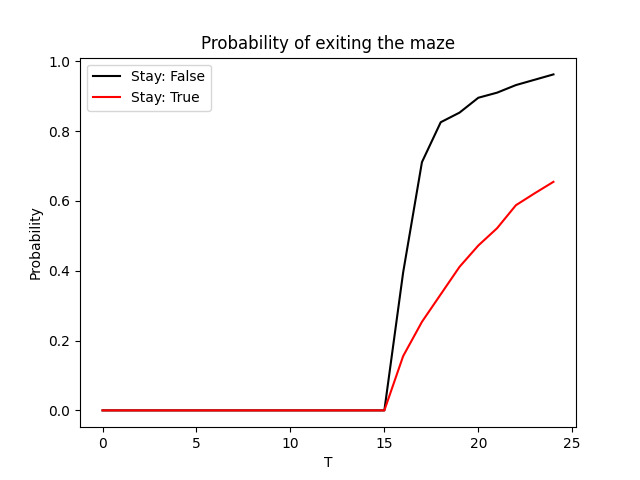
\includegraphics[width=0.8\textwidth]{Lab_1/images/problem_1/probability_of_exiting_the_maze_3.png}
    \caption{\small Probability of exiting the maze as a function of T, with 10 000 runs for each $t=1,2,3,...,25$.}
    \label{fig:probability_exiting}
\end{figure}

If the minotaur is allowed to stand still, the minotaur can block us from getting to the goal. And thus the probability of getting out alive is decreased as can be seen in Figure \ref{fig:probability_exiting}.


\subsection*{C)}
By assuming that the players life is geometrically distributed with mean $E[T] = 30$ the discount factor $\lambda$ is derived by $E[T] =  \frac{1}{1 - \lambda} \Rightarrow \lambda = 1 - \frac{1}{30}$. When using $\lambda = 1 - \frac{1}{30}$ and $\epsilon = 0.01$ the probability of getting out alive using this policy, for 10 000 games, where equal to 1, i.e. the player where able to get out alive successfully every single game that it played.









\section*{Problem 2: \\
        Robbing Banks}
        
        
\subsection*{A)}
The problem can me modelled as an MDP such that, the number of states is depending on the grid space and the robber and police position, e.g. $S = \{((R_x, R_y),(P_x, P_y) )\} $ where $R_x$ and $R_y$ is the robber and $P_x$ and $P_y$ the police position x and y position within the grid. The state space can be divided into $S = {S_a, S_u}$ where $S_a$ is the allowed states and $S_u$ is the unreachable states, such as out-of-boundary.


\textbf{State space:}\\
$S = \{((R_x, R_y),(P_x, P_y) )\} $, 324 number of states. 

\textbf{Actions}: \\
The actions can be as described in the lab instructions as left, right, up, down or stay at the current position, $A = \{ A_{left}, A_{right}, A_{up}, A_{down}, A_{stay} \}$. 

\textbf{Rewards:} \\
Caught: $r(R_x = P_x , R_y = P_y |s,a) = -100 $\\ 
Robbing: $r(R_x = B_x , R_y = B_y |s,a) = 0 $, where $B_x$, $B_y$ is the goal position\\
Out-of-boundary: $r(s'\in S_u |s,a) = -\infty $

\textbf{Transition Probabilities}:\\
$P_t(s' \in S_a |s,a) = 1/n$, where n is the number of possible moves for the Police(n is either $3$ or $2$) as stated in the lab instruction, and \\$P_t(s \in S_u |s,a) = 0$ if trying to take an action that is out-of-boundary. 

        


\subsection*{B)}

\begin{figure}[H]
    \centering
    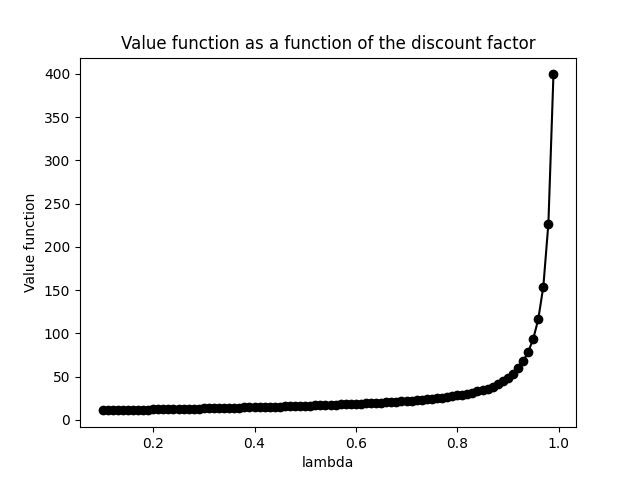
\includegraphics[width=0.8\textwidth]{Lab_1/images/problem_2/valueFunction.png}
    \caption{\small The Value function(evaluated at the initial state) as a function of the discount factor(\lambda). }
    \label{fig:Valfunc}
\end{figure}




\noindent 
In Figure \ref{fig:Valfunc} the value function evaluated in the initial state is increasing for increasing values of lambda. This was expected because with an larger $\lambda$ we take more future rewards into account.   




\begin{figure}[H]
    \centering
    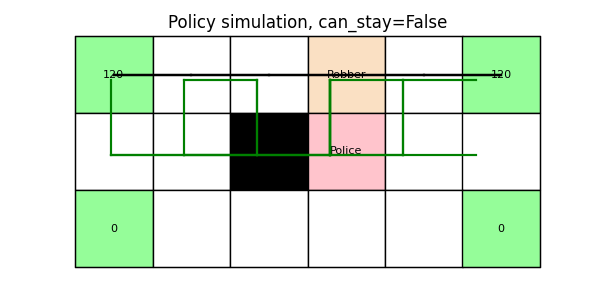
\includegraphics[width=0.8\textwidth]{Lab_1/images/problem_2/cityRun_ValIter_Nov-25-2020_11-55-18.png}
    \caption{\small Illustration of the optimal policy for \lambda > 0.85  }
    \label{fig:optpol1}
\end{figure}

As seen in Figure \ref{fig:optpol1} compared to Figure \ref{fig:optpol2} the optimal policy changes depending on $\lambda$. With $\lambda > 0.85$ the optimal policy is the behaviour from Figure \ref{fig:optpol1}, i.e. just robbing and moving between Bank1 and Bank4. 
With $\lambda \leq 0.85$ we obtain the optimal policy from Figure \ref{fig:optpol2}, i.e. just robbing and moving between Bank1 and Bank2. 



\end{document}
